\documentclass[11pt,a4paper]{article}

% Packages
\usepackage[utf8]{inputenc}
\usepackage[spanish, es-tabla]{babel}
\usepackage{parskip}
\usepackage{enumerate}
\usepackage{graphicx}
\usepackage{subfigure}
\usepackage{float}
\usepackage{amsmath}


\usepackage[bookmarks=true,
					 bookmarksnumbered=false,
					 bookmarksopen=false,
					 colorlinks=true,
					 allcolors=blue,
					 urlcolor=blue]{hyperref}

\usepackage[ruled]{algorithm2e}
\SetKwInOut{Parameter}{parameter}

\usepackage{array}
\newcolumntype{N}{>{\centering\arraybackslash}m{0.5cm}}
\newcolumntype{M}{>{\centering\arraybackslash}m{1cm}}

\usepackage[left=2cm, right=2cm, top=2cm, bottom=2cm]{geometry}

\begin{document}\pagenumbering{arabic}
\begin{titlepage}
\centering
\includegraphics[width=0.15\textwidth]{/Users/pedrors/Desktop/DGIIM/Latex/UGR}\par\vspace{1cm}
{\scshape\LARGE Universidad de Granada \par}
\vspace{1cm}
{\Huge\bfseries Práctica 1.b\par}
{\Large\bfseries Técnicas de Búsquedad Local y Algoritmos Greedy para el Problema del aprendizaje de Pesos en Características\par}
\vspace{1.5cm}
{\huge\bfseries Metaheurísticas\par}
{\large\bfseries Grupo 2 (Lunes)\par}
\vspace{2cm}
{\Large\itshape Pedro Ramos Suárez\par}
{\large\itshape 76591270M\par}
{\large\itshape pedrors@correo.ugr.es\par}
\vfill
Doble Grado de Ingeniería Informática y Matemáticas
\vfill
{\large 4 de abril de 2022\par}
\author{A}
\end{titlepage}

\tableofcontents
\newpage
\section{Problema de Aprendizaje de Pesos en Características}

\subsection{Descripción del problema}

El problema consiste en optimizar el rendimiento de un clasificador basado en el vecino más cercano a partir de la inclusión de pesos asociados a las características del problema.

El clasificador utilizado es el 1-NN (1 vecino más cercano), el cuál consiste en asignar a cada nuevo la misma etiqueta que a su vecino más cercano. Para ello, utilizamos la distancia euclídea modificada por unos pesos asociados a cada característica:
$$d(e_{1}, e_{2}) = (\sum_{i=1}^{n} w_{i} \cdot (e_{1}^{i} - e_{2}^{i})^{2})^{\frac{1}{2}}$$
donde $n$ es el número de características de los datos, y $W = (w_{1}, \dots, w_{n})$ el vector de números reales entre 0 y 1 que define el peso que pondera cada una de las características.

La variante que intentaremos optimizar será la agregación, que combina tanto la precisión como la complejidad del clasificador, definida como:
\begin{equation} \label{eq:objetivo}
\text{Agregación}(W) = \alpha \cdot \text{Tasa\_clas}(W) + (1 - \alpha) \cdot \text{Tasa\_red}(W)
\end{equation}
donde:
\begin{equation} \label{eq:clas}
\text{Tasa\_clas} = 100 \cdot \frac{\text{nº de instancias bien clasificadas en T}}{\text{nº de instancias en T}}
\end{equation}
\begin{equation} \label{eq:red}
\text{Tasa\_red} = 100 \cdot \frac{\text{nº de valores } w_{i} < 0.1}{\text{nº de características}}
\end{equation}

siendo $T$ el conjunto de datos sobre los que se evalúa el clasificador, y $\alpha$ es un número real entre 0 y 1 que pondera la importancia entre acierto y la reducción de la solución.

\subsection{Datos utilizados}

Los datos utilizados serán:
\begin{enumerate}
\item \textbf{Ionosphere}: Conjunto de datos de radar, formado por 351 ejemplos con 34 características clasificados en dos clases.
\item \textbf{Parkinsons}: Conjunto de datos orientados a distinguir entre la presencia y ausencia de la enfermedad de Parkinson en una serie de pacientes, formado por 195 ejemplos con 22 características clasificados en dos clases.
\item \textbf{Spectf-heart}: Conjunto de datos de detección de enfermedades cardíacas a partir de imágenes médicas de termografía computerizada del corazón, formada por 349 ejemplos con 44 características clasificados en dos clases.
\end{enumerate}

\newpage
\section{Aplicación de los algoritmos}
Todos los algoritmos utilizados para resolver este problema tienen como entrada la matriz de datos de las características $D = (k \times n)$, y el vector de etiquetas asociadas a dicha matriz $y = (y_{1}, \dots, y_{k})$, donde $k$ es el número de ejemplos, y $n$ el número de características. Dependiendo del algoritmo, estos datos pueden ser todos los leídos, o sólo un subconjunto de entrenamiento.

Para representar las soluciones, utilizaremos un vector de números reales entre 0 y 1, $W = (w_{1}, \dot, w_{n})$, que define el peso que pondera cada una de las características.

La evaluación de la calidad de una solución se hará como indicada en \eqref{eq:objetivo}, tomando como $\alpha = 0.5$, es decir, dándole la misma importancia al acierto y a la reducción de las características, por lo que será de la forma:
$$\text{Agregación}(W) = 0.5 \cdot \text{Tasa\_clas}(W) + 0.5 \cdot \text{Tasa\_red}(W) = \frac{\text{Tasa\_clas}(W) + \text{Tasa\_red}(W)}{2}$$

\subsection{Algoritmos para evaluar las soluciones}

El pseudocódigo de la función para calcular la tasa de clasificación es: \\
\begin{algorithm}[H]
	\caption{{\sc Tasa\_Clas} calcula la tasa de clasificación de una solución.}
	\KwIn{El conjunto de etiquetas reales $Y$.}
	\KwIn{El conjunto de etiquetas obtenidas de la predicción del vecino más cercano $P$.}
	\KwOut{La tasa de clasificación como se describe en \eqref{eq:clas}.}
	
	$clas \gets 0$ \;
	\For{$i=0$ \textbf{to} $length(Y)$} {
		\If{$Y[i] = P[i]$} {
			$clas \gets clas + 1$ \;
		}
	}
	$output \gets clas / length(Y)$ \;
	\Return{$output$} \;
\end{algorithm}

El pseudocódigo de la función para calcular la tasa de reducción es: \\
\begin{algorithm}[H]
	\caption{{\sc Tasa\_Red} calcula la tasa de reducción de una solución.}
	\KwIn{El conjunto de pesos $W$.}
	\KwIn{El conjunto de etiquetas obtenidas de la predicción del vecino más cercano $P$.}
	\KwOut{La tasa de clasificación como se describe en \eqref{eq:red}.}
	
	$red \gets 0$ \;
	\For{$w$ \textbf{in} $W$} {
		\If{$w < 0.1$} {
			$red \gets red + 1$ \;
		}
	}
	$output \gets red / length(W)$ \;
	\Return{$output$} \;
\end{algorithm}

Por último, el pseudocódigo de la función de agregación obtenido a partir de la tasa de clasificación y la tasa de reducción es: \\
\begin{algorithm}[H]
	\caption{{\sc Agregacion} calcula la agregación de una solución.}
	\KwIn{El conjunto de pesos $W$.}
	\KwOut{La agregación como se describe en \eqref{eq:objetivo}.}
	
	$clas \gets \operatorname{tasa\_clas}(W)$ \;
	$red \gets \operatorname{tasa\_red}(W)$ \;
	$output \gets (clas + red)/2$ \;
	\Return{$output$} \;
\end{algorithm}

\subsection{Algoritmos para calcular las distancias}

Utilizaremos la distancia euclídea o una variante que modifica la importancia de cada componente según los pesos.

El pseudocódigo para la distancia euclídea es: \\
\begin{algorithm}[H]
	\caption{{\sc Eulcidean} calcula la distancia entre dos puntos.}
	\KwIn{Un vector con las coordenadas del primer punto $P$.}
	\KwIn{Un vector con las coordenadas del segundo punto $Q$.}
	\KwOut{La distancia entre los dos puntos.}
	
	$dist \gets 0$ \;
	\For{$i=0$ \textbf{to} $length(P)$} {
		$dist \gets dist + (P[i] - Q[i])^{2}$ \;
	}
	$output \gets sqrt(dist)$ \;
	\Return{$output$} \;
\end{algorithm}

El pseudocódigo para la distancia euclídea modificada por el vector de pesos es: \\
\begin{algorithm}[H]
	\caption{{\sc Weighted\_Eulcidean} calcula la distancia entre dos puntos.}
	\KwIn{Un vector de pesos $W$.}
	\KwIn{Un vector con las coordenadas del primer punto $P$.}
	\KwIn{Un vector con las coordenadas del segundo punto $Q$.}
	\KwOut{La distancia entre los dos puntos.}
	
	$dist \gets 0$ \;
	\For{$i=0$ \textbf{to} $length(W)$} {
		$dist \gets dist + W[i] (P[i] - Q[i])^{2}$ \;
	}
	$output \gets sqrt(dist)$ \;
	\Return{$output$} \;
\end{algorithm}

\subsection{Algoritmos para predecir las etiquetas}

Tenemos dos casos:
\begin{enumerate}
\item El conjunto de datos está dividido en entrenamiento y test. Entonces predeciremos las etiquetas del conjunto de test a partir de los resultados obtenidos en entrenamiento.
\item Los datos no están divididos en entrenamiento y test. Entonces aplicaremos el algoritmo \emph{leave-one-out}, que predice una etiqueta a partir de todos los demás datos.
\end{enumerate}

Para el pseudocódigo utilizaremos la versión de la distancia euclídea con pesos. Sin embargo, el caso que no los utiliza sería casi idéntico, pero sin tomar el vector de pesos como entrada, y utilizando la función \emph{euclidean} en lugar de \emph{weighted\_euclidean}.

El pseudocódigo para el primer caso, en el que tenemos los datos separados en entrenamiento y test, es: \\
\begin{algorithm}[H] \label{alg:predictlabel}
	\caption{{\sc Predict\_Label} predice las etiquetas.}
	\KwIn{Una matriz de datos de test $X\_test$.}
	\KwIn{Una matriz de datos de entrenamiento $X$.}
	\KwIn{Un vector con las etiquetas de entrenamiento $Y$.}
	\KwIn{El vector de pesos $W$.}
	\KwOut{Un vector con la predicción de etiquetas de los datos de test.}
	
	$Y\_pred \gets \{\}$ \;
	\For{$x$ \textbf{in} $X\_test$} {
		$min\_dist \gets length(x)$ \;
		$neighbour \gets 0$ \;
		\For{$i=0$ \textbf{to} $length(X)$} {
			$dist \gets \operatorname{weighted\_euclidean}(x, X[i], W)$ \;
			\If{$dist < min\_dist$} {
				$min\_dist \gets dist$ \;
				$neightbour \gets i$ \;
			}
		}
		$Y\_pred \gets Y\_pred \cup \{neighbour\}$ \;
	}
	\Return{$Y\_pred$} \;
\end{algorithm}

Nótese que inicializamos la distancia mínima como el la longitud de $x$, es decir, el número de características. Esto se debe a que como los datos están normalizados, la distancia siempre será menor.

El pseudocódigo para el segundo caso, \emph{leave-one-out}, en el que tenemos un único conjunto de datos, es:
\begin{algorithm}[H] \label{alg:leaveoneout}
	\caption{{\sc Leave\_One\_Out} predice las etiquetas.}
	\KwIn{Una matriz de datos $X$.}
	\KwIn{Un vector con las etiquetas $Y$.}
	\KwIn{El vector de pesos $W$.}
	\KwOut{Un vector con la predicción de etiquetas.}
	
	$Y\_pred \gets \{\}$ \;
	\For{$x$ \textbf{in} $X$} {
		$min\_dist \gets length(x)$ \;
		$neighbour \gets 0$ \;
		\For{$i=0$ \textbf{to} $length(X)$} {
			\If{$x \neq X[i]$} {
				$dist \gets \operatorname{weighted\_euclidean}(x, X[i], W)$ \;
				\If{$dist < min\_dist$} {
					$min\_dist \gets dist$ \;
					$neightbour \gets i$ \;
				}
			}
		}
		$Y\_pred \gets Y\_pred \cup \{neighbour\}$ \;
	}
	\Return{$Y\_pred$} \;
\end{algorithm}

\subsection{Otros algoritmos}

Por último, sólo nos queda un algoritmo que merece la pena mencionar, que es el que separa los datos en entrenamiento: \\
\begin{algorithm}[H]
	\caption{{\sc Train\_Test\_Split} divide los datos en entrenamiento y test.}
	\KwIn{Una matriz de datos $X$.}
	\KwIn{Un vector con las etiquetas $Y$.}
	\KwIn{Un entero que indica el número de conjuntos en el que dividir los datos $n$.}
	\KwIn{Un entero que indica qué conjunto es de test y cuáles de entrenamiento $k$.}
	\KwOut{Un vector con los datos de entrenamiento.}
	\KwOut{Un vector con los datos de test.}
	\KwOut{Un vector con las etiquetas de entrenamiento.}
	\KwOut{Un vector con las etiquetas de test.}
	
	$X\_train \gets \{\}$ \;
	$X\_test \gets \{\}$ \;
	$Y\_train \gets \{\}$ \;
	$Y\_test \gets \{\}$ \;
	$size \gets length(X) / n$ \;
	$remain \gets length(X) \% n$ \;
	\uIf{$k < remain$} {
		$begin \gets (size + 1)$ \;
		$end \gets begin + (size + 1)$ \;
	} \uElseIf{$k == remain$} {
		$begin \gets (size + 1)$ \;
		$end \gets begin + size$ \;
	} \Else {
		$begin \gets size$ \;
		$end \gets begin + size$ \;
	}
	\For{$i=0$ \textbf{to} $length(X)$} {
		\uIf{$i < begin$ \textbf{or} $i > begin$} {
			$X\_train \gets X\_train \cup X[i]$ \;
			$Y\_train \gets Y\_train \cup Y[i]$ \;
		} \Else{
			$X\_test \gets X\_test \cup X[i]$ \;
			$Y\_test \gets Y\_test \cup Y[i]$ \;
		}
	}
	\Return{$X\_train$} \;
	\Return{$X\_test$} \;
	\Return{$Y\_train$} \;
	\Return{$Y\_test$} \;
\end{algorithm}

En caso de que el número de datos sea múltiplo del número de particiones, todas estas tendrán el mismo tamaño. En caso de que no lo sea, los primeros conjuntos de test tendrán un elemento extra.

\newpage
\section{Descripción de los algoritmos}

\subsection{Búsqueda Local}

Procedemos al algoritmo de Búsqueda Local, el objetivo de esta práctica. Generamos nuevas soluciones modificando de manera aleatoria el vector de pesos. Debido a esto, hay infinitas posibles nuevas soluciones, por lo que utilizamos la técnica del Primero Mejor, con la cuál tomamos una nueva solución si es mejor que la actual.

Iniciaremos el algoritmo con una solución aleatoria generando cada componente a partir de una distribución uniforme entre 0 y 1, utilizando la función: \\
\begin{algorithm}[H]
	\caption{{\sc Random\_Sol} genera una solución aleatoria.}
	\KwIn{El tamaño del vector de pesos $n$.}
	\KwOut{Un vector con una solución aleatoria.}
	
	$W \gets \{\}$ \;
	\For{$i=0$ \textbf{to} $length(X[0])$} {
		$e \gets$ elemento aleatorio de una distribución uniforme \;
		\If{$e < 0.1$} {
			$e \gets 0$ \;
		}
		$W \gets W \cup \{e\}$ \;
	}
	\Return{$W$} \;
\end{algorithm}

En cada paso de la exploración modificamos una componente del vector de pesos distinta sin repetición hasta encontrar mejora (técnica del Primero Mejor) o hasta modificar todas las componentes sin conseguir una mejora, momento en el cual se comienza de nuevo la exploración. Para ello, necesitamos una función que nos de el orden en el que aplicar las modificaciones de forma aleatoria: \\
\begin{algorithm}[H]
	\caption{{\sc Permutation} genera una permutación.}
	\KwIn{El tamaño del vector de pesos $n$.}
	\KwOut{Un vector con la permutación.}
	
	$perm \gets \{0, \dots, n-1\}$ \;
	$perm \gets \operatorname{shuffle}(perm)$ \;
	\Return{$perm$} \;
\end{algorithm}

Continuaremos generando candidatos hasta realizar un total de 15000 iteraciones (contando como iteración cada vez que modificamos una componente del vector de pesos), o 20 iteraciones sin obtener una solución mejor (contando como iteración modificar todas las componentes del vector de pesos).

Cabe mencionar que para obtener el número de características utilizamos \emph{length(X[0])}, ya que, a menos que usemos un conjunto vacío (caso que no tiene sentido), siempre tendremos un elemento en esa posición.

Con todo esto, el algoritmo de búsqueda local queda de la forma: \\
\begin{algorithm}[H]
	\caption{{\sc LocalSearch}}
	\KwIn{Una matriz de datos $X$.}
	\KwIn{Un vector de etiquetas $Y$.}
	\KwOut{Un vector de pesos.}
	
	$iteration \gets 0$ \;
	$iteration\_mod \gets 0$ \;
	$W \gets \operatorname{random\_sol}(length(X[0]))$ \;
	\While{$iteration < 15000$ \textbf{and} $iteration\_mod < 20$} {
		$modified \gets false$ \;
		$perm \gets \operatorname{permutation}(length(W))$ \;
		
		\For{$i==0$ \textbf{to} $length(W)$ \textbf{and not} $modified$ \textbf{and} $iteration < 15000$} {
			$s \gets$ elemento aleatorio de una distribución normal de media 0 y varianza 0.3 \;
			$neighbour \gets \operatorname{copy}(W)$ \;
			$neighbour[i] \gets neighbour[i] + s$ \;
			\uIf{$neighbour[i] > 1$} {
				$neighbour[i] \gets 1$ \;
			} \ElseIf{$neighbour[i] < 0.1$} {
				$neighbour[i] \gets 0$ \;
			}
			
			\If{$\operatorname{agregation}(neighbour) > \operatorname{agregation}(W)$} {
				$W \gets neighbour$ \;
				$modified \gets true$ \;
			}
			$iteration \gets iteration + 1$ \;
		} 
		\uIf{$modified$} {
			$iteration\_mod \gets 0$ \;
		} \Else{
			$iteration\_mod \gets iteration\_mod + 1$ \;
		}
	}
	\Return{$W$} \;
\end{algorithm}

\newpage
\section{Algoritmos de comparación}

\subsection{1-NN}

El primer algoritmo que utilizaremos para comparar la eficacia del algoritmo es \emph{1-NN}, que es el algoritmo \textbf{k-NN} ($k$ nearest neighbours) con $k = 1$, es decir, con un sólo vecino.

Los demás algoritmos son una versión modificada de este, en los que modificamos la distancia euclídea con un vector de pesos. Debido a ello, como no tenemos vector de pesos, no estamos realizando ninguna optimización, y los resultados solo dependen de los datos de entrada, por lo que no tiene sentido dividir los datos en entrenamiento y test (ya que no ``entrenamos''), así que usamos la técnica \emph{leave-one-out}.

El funcionamiento del algoritmo ya ha sido explicado en el algoritmo \ref{alg:leaveoneout}.

\subsection{Greedy: RELIEF}

El principal algoritmo que utilizaremos para comparar la eficacia es el \emph{greedy} \textbf{RELIEF}, que genera un vector de pesos a partir de las distancias de cada ejemplo a su \emph{enemigo}, que es el ejemplo de diferente clase más cercano, y a su \emph{amigo} más cercano, que es el ejemplo de la misma clase más cercano.

El algoritmo aumentará el peso de las características que mejor separan a ejemplos enemigos, y reduce el peso en las que separan a amigos. El incremento es proporcional a la distancia entre los ejemplos en cada característica.

\begin{algorithm}[H]
	\caption{{\sc RELIEF}}
	\KwIn{Una matriz de datos $X$.}
	\KwIn{Un vector de etiquetas $Y$.}
	\KwOut{Un vector de pesos.}
	
	$W \gets \{0, 0, \dots, 0\}$ \tcp{Tantos ceros como carcaterísticas tengan los datos.}
	\For{$i=0$ \textbf{to} $length(X)$} {
		$ind\_enemy \gets i$ \;
		$ind\_friend \gets i$ \;
		$dist\_enemy \gets length(X[0])$ \tcp{Al normalizar los datos, la distancia máxima}
		$dist\_friend \gets length(X[0])$ \tcp{es $\sqrt{k}<k$, siendo $k$ el número de características}
		\For{$j=0$ \textbf{to} $length(X)$} {
			\If{$i \neq j$} {
				\uIf{$X[i] == X[j]$ \textbf{and} $\operatorname{weighted\_euclidean}(X[i], X[j], W) < dist\_friend$} {
					$ind\_friend \gets j$ \;
					$dist\_friend \gets \operatorname{weighted\_euclidean}(X[i], X[j], W)$ \;
				} \ElseIf{$X[i] \neq X[j]$ \textbf{and} $\operatorname{weighted\_euclidean}(X[i], X[j], W) < dist\_enemy$} {
					$ind\_enemy \gets j$ \;
					$dist\_enemy \gets \operatorname{weighted\_euclidean}(X[i], X[j], W)$ \;
				}
			}
		}
		\For{$j=0$ \textbf{to} $length(X[0])$} {
			$w[j] \gets |X[i][j] - x[ind\_enemy][j]| - |X[i][j] - X[ind\_friend][j]|$ \;
		}
	}
	$W \gets \operatorname{normalize\_weight}(W)$ \;
	\Return{$W$} \;
\end{algorithm}
donde \emph{normalize\_weight} es la función que normaliza los valores del vector de pesos, haciendo que estén entre 0 y 1, y aplica la reducción, eliminando aquellos valores que están por debajo de 0.1, es decir: \\
\begin{algorithm}[H]
	\caption{{\sc Normalize\_Weight} normaliza y aplica reducción al vector de pesos.}
	\KwIn{El vector de pesos $W$.}
	\KwOut{El vector de pesos normalizado.}
	
	$max\_w \gets w[0]$ \;
	\For{$k$ \textbf{in} $W$} {
		\If{$k > max\_w$} {
			$max\_w \gets w$ \;
		}
	}
	\For{$k$ \textbf{in} $W$} {
		\uIf{$k < 0.1$} {
			$k \gets 0$ \;
		} \Else {
			$k \gets k/max\_w$ \;
		}
	}
	\Return{$W$} \;
\end{algorithm}

\newpage
\section{Desarrollo de la práctica}

La práctica ha sido implementada en C++, utilizando las siguientes bibliotecas:
\begin{itemize}
\item \textbf{iostream}: Para salida de datos por pantalla.
\item \textbf{fstream}: Para lectura y escritura en ficheros.
\item \textbf{sstream}: Para lectura y escritura en ficheros.
\item \textbf{string}: Para lectura y escritura en ficheros.
\item \textbf{vector}: Para almacenar los datos en un vector de vectores (que funciona como una matriz), y las etiquetas y los pesos en un vector.
\item \textbf{math.h}: Para el calculo de la raíz cuadrada para la distancia euclídea.
\item \textbf{stdlib.h}: Para la generación de distribuciones aleatorios.
\item \textbf{random}: Para la generación de aleatorios.
\item \textbf{chrono}: Para calcular el tiempo de ejecución utilizando \emph{system\_clock}.
\item \textbf{regex}: Para modificar strings. Utilizado únicamente en la búsqueda local para poder exportar datos y representarlos en gráficas.
\end{itemize}

Los ficheros están almacenados en los siguientes directorios:
\begin{itemize}
\item \textbf{bin}: Contiene los archivos ejecutables.
\item \textbf{src}: Contiene los archivos con el código.
\item \textbf{data}: Contiene los ficheros con los datos.
\item \textbf{graph}: Contiene un archivo de \emph{python}, y dos carpetas. En la primera de ellas, \emph{data}, se almacenan datos para representarlos. El archivo \emph{graphPlotter.py} lee todos los archivos que haya en este carpeta, y crea sus gráficas, guardándolos en la segunda carpeta, \emph{plots}. Esto está más desarrollado en el siguiente apartado.
\end{itemize}

Dentro de los ficheros, tenemos las constantes:
\begin{itemize}
\item \textbf{SEED}: Usado en los tres algoritmos. Contiene la semilla usada para las generaciones aleatorias. Por defecto, 0.
\item \textbf{FOLDS}: Usado en \emph{knn} y \emph{localSearch}. Contiene el número de particiones en las que dividir el conjunto de datos para entrenamiento y test usando \emph{k-folds cross validation}.
Tomará uno de estos conjuntos como test, y el resto como entrenamiento. Por defecto, 5.
\item \textbf{REDUCCTION}: Usado en \emph{knn} y \emph{localSearch}. Contiene el umbral por debajo del cual los pesos se consideran como 0. Por defecto, 0.1.
\item \textbf{EXPORT}: Usado exclusivamente en \emph{localSearch}. Determina si se almacenan datos para su posterior representación en gráficas (explicado más en detalle en el siguiente apartado). Por defecto, para reducir el tiempo de ejecución, no almacena datos, esto es, inicializamos a \emph{false}.
\end{itemize}

\subsection{Representación en gráficas} \label{sec:graphs}

Un resultado interesante que se puede observar es como evolucionan la tasa de clasificación, reducción y agregación con las iteraciones en el algoritmo de búsqueda local. Sin embargo, en C++ no existe ninguna función o biblioteca que facilite la representación en gráficas.

Para solucionar esto, definimos una nueva función llamada \emph{export\_localSearch}, que tiene el mismo funcionamiento que \emph{localSearch}, pero cada vez que se encuentra una mejor solución, almacena la iteración y las tasas en un fichero en el directorio \emph{graph\/data}. Esta definida como una nueva función ya que, si añadiésemos comprobaciones o salida a un fichero, aumentaríamos el tiempo de ejecución.

En el directorio \emph{graph}, tenemos además un archivo llamado \emph{graphPlotter.py}, que es un archivo en \emph{Python} que lee todos los ficheros de \emph{graph\/data}, crea las gráficas usando \emph{matplotlib}, y las almacena como imágenes en \emph{graph\/plots}.

Con esto, podemos tener gráficas como la siguiente:
\begin{figure}[H]
	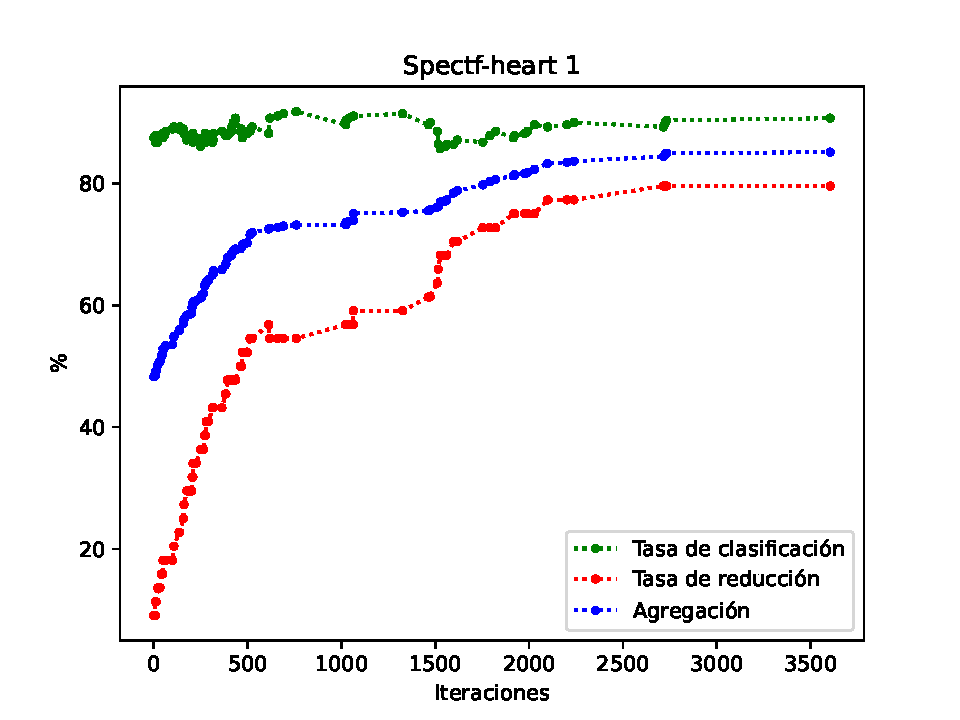
\includegraphics[scale=1]{../FUENTES/graph/plots/spectf-heart1.pdf}
	\caption{Ejemplo de gráfica obtenida}
\end{figure}
Nótese que esta gráfica es un suavizado de la gráfica real, ya que en la gráfica real las tasas no cambiaría hasta encontrar una mejor solución, momento en el que ocurriría un salto, por lo que tendríamos funciones a saltos, en lugar de continuas. Sin embargo, para una ``mejor'' representación, las tratamos como funciones continuas.

Todas las gráficas, incluido este ejemplo, están incluidas en la sección de resultados.

Para eliminar todos los datos y las gráficas obtenidas, podemos ejecutar \emph{make fullclean}, que elimina tanto los ejecutables como los datos en las carpetas de \emph{graph}.

\subsection{Manual de usuario}

Para obtener los ficheros ejecutables, sólo tenemos que realizar el comando \emph{make}, el cuál compila el código fuente usando optimización \emph{-O2}.

Los ficheros ejecutables son:
\begin{itemize}
\item \textbf{knn}: Implementación del algoritmo \emph{k-NN}, con $k = 1$.
\item \textbf{Greedy}: Implementación del algoritmo greedy \emph{RELIEF}.
\item \textbf{LocalSearch}: Implementación del algoritmo Búsqueda Local.
\end{itemize}

Los archivos de código contienen una explicación de todas las funciones, así como de los parámetros que toman de entrada y de salida. Además, al comienzo de cada uno de ellos, están definidas las constantes en caso de que se deseen modificar.

Toda la parte de generación de gráficas crea los archivos necesarios automáticamente, y con \emph{make fullclean}, todos son eliminados (excepto el archivo de \emph{Python}).

Todos requieren el uso de un fichero de entrada, e imprimen por pantalla los resultados obtenidos. En el caso de \emph{RELIEF} y la Búsqueda Local, como separamos los datos en entrenamiento y test, imprimen los resultados para cada uno de los conjuntos de test.

Por ejemplo, si queremos ejecutar el algoritmo \emph{localSearch} con los datos de \emph{ionosphere.arff}, sería:
\begin{verbatim}
bin/localSearch data/ionosphere.arff
\end{verbatim}

\newpage
\section{Experimentos y análisis de resultados}
Todos los resultados se han obtenido en un ordenador con las siguientes especificaciones:
\begin{itemize}
\item Sistema operativo: macOS Montery.
\item Procesador: 1,6 GHz Intel Core i5 de doble núcleo.
\item Memoria: 16 GB 2133 MHz LPDDR3.
\item Gráficos: Intel UHD Graphics 617 1536 MB.
\end{itemize}

\subsection{Resultados}

En todos los resultados, el tiempo es en segundos.

Los resultados obtenidos con el algoritmo \emph{greedy RELIEF} son:
\begin{table}[H]
\centering \tiny
\begin{tabular}{ M || c | c | c | c || c | c | c | c || c | c | c | c |}
\cline{2-13}
\multicolumn{1}{c|}{ } & \multicolumn{4}{c||}{Ozone} & \multicolumn{4}{c||}{Parkinsons} & \multicolumn{4}{c|}{Spectf-heart} \\ \cline{2-13}
\multicolumn{1}{c|}{ } & \%\_clas & \%\_red & Agr. & T & \%\_clas & \%\_red & Agr. & T & \%\_clas & \%\_red & Agr. & T \\ \hline
\multicolumn{1}{|c||}{Partición 1} & 90.14 & 2.94 & 46.54 & 0.02 & 94.87 & 0.00 & 47.44 & 0.01 & 77.14 & 0.00 & 38.57 & 0.02 \\ \hline
\multicolumn{1}{|c||}{Partición 2} & 70.00 & 2.94 & 36.47 & 0.02 & 100.00 & 0.00 & 50.00 & 0.01 & 84.29 & 0.00 & 42.14 & 0.02 \\ \hline
\multicolumn{1}{|c||}{Partición 3} & 67.14 & 2.94 & 35.04 & 0.02 & 94.87 & 0.00 & 47.44 & 0.01 & 77.14 & 0.00 & 38.57 & 0.02 \\ \hline
\multicolumn{1}{|c||}{Partición 4} & 68.57 & 2.94 & 35.76 & 0.02 & 97.44 & 0.00 & 48.72 & 0.01 & 92.86 & 0.00 & 46.43 & 0.02 \\ \hline
\multicolumn{1}{|c||}{Partición 5} & 67.14 & 2.94 & 35.04 & 0.02 & 94.87 & 0.00 & 47.44 & 0.01 & 86.96 & 0.00 & 43.48 & 0.02 \\ \hline \hline
\multicolumn{1}{|c||}{Media} & 72.60 & 2.94 & 37.77 & 0.02 & 96.41 & 0.00 & 48.21 & 0.01 & 83.68 & 0.00 & 41.84 & 0.02 \\ \hline
\end{tabular}
\caption{Tabla con los resultados del algoritmo greedy RELIEF.}
\end{table}

Los resultados obtenidos con el algoritmo \emph{localSearch} son:
\begin{table}[H]
\centering \tiny
\begin{tabular}{ M || c | c | c | c || c | c | c | c || c | c | c | c |}
\cline{2-13}
\multicolumn{1}{c|}{ } & \multicolumn{4}{c||}{Ozone} & \multicolumn{4}{c||}{Parkinsons} & \multicolumn{4}{c|}{Spectf-heart} \\ \cline{2-13}
\multicolumn{1}{c|}{ } & \%\_clas & \%\_red & Agr. & T & \%\_clas & \%\_red & Agr. & T & \%\_clas & \%\_red & Agr. & T \\ \hline
\multicolumn{1}{|c||}{Partición 1} & 92.96 & 88.24 & 90.60 & 25.71 & 87.18 & 83.36 & 86.77 & 6.61 & 74.29 & 79.55 & 76.92 & 59.97 \\ \hline
\multicolumn{1}{|c||}{Partición 2} & 88.67 & 79.41 & 84.04 & 38.19 & 89.74 & 68.18 & 78.96 & 4.59 & 85.71 & 81.82 & 83.77 & 80.71 \\ \hline
\multicolumn{1}{|c||}{Partición 3} & 84.29 & 88.24 & 86.26 & 45.87 & 89.75 & 81.82 & 85.78 & 3.86 & 80.00 & 72.73 & 76.36 & 41.19 \\ \hline
\multicolumn{1}{|c||}{Partición 4} & 78.57 & 61.76 & 70.17 & 27.53 & 92.31 & 72.73 & 82.52 & 2.97 & 87.14 & 79.55 & 83.34 & 37.09 \\ \hline
\multicolumn{1}{|c||}{Partición 5} & 80.00 & 85.29 & 82.65 & 24.81 & 87.18 & 86.36 & 86.77 & 5.44 & 82.61 & 75.00 & 78.80 & 42.40 \\ \hline \hline
\multicolumn{1}{|c||}{Media} & 84.90 & 80.59 & 82.74 & 32.42 & 89.23 & 79.09 & 84.16 & 4.69 & 81.95 & 77.73 & 79.84 & 52.27 \\ \hline
\end{tabular}
\caption{Tabla con los resultados del algoritmo localSearch.}
\end{table}

Finalmente, los resultados globales son:
\begin{table}[H] \label{tab:global}
\centering \tiny
\begin{tabular}{ M || c | c | c | c || c | c | c | c || c | c | c | c |}
\cline{2-13}
\multicolumn{1}{c|}{ } & \multicolumn{4}{c||}{Ozone} & \multicolumn{4}{c||}{Parkinsons} & \multicolumn{4}{c|}{Spectf-heart} \\ \cline{2-13}
\multicolumn{1}{c|}{ } & \%\_clas & \%\_red & Agr. & T & \%\_clas & \%\_red & Agr. & T & \%\_clas & \%\_red & Agr. & T \\ \hline
\multicolumn{1}{|c||}{1-NN} & 86.89 & 0.00 & 43.45 & 0.02 & 96.41 & 0.00 & 48.21 & 0.00 & 86.25 & 0.00 & 43.12 & 0.02 \\ \hline
\multicolumn{1}{|c||}{RELIEF} & 72.60 & 2.94 & 37.77 & 0.02 & 96.41 & 0.00 & 48.21 & 0.01 & 83.68 & 0.00 & 41.84 & 0.02 \\ \hline
\multicolumn{1}{|c||}{BL} & 84.90 & 80.59 & 82.74 & 32.42 & 89.23 & 79.09 & 84.16 & 4.69 & 81.95 & 77.73 & 79.84 & 52.27 \\ \hline
\end{tabular}
\caption{Tabla con los resultados globales en el problema APC.}
\end{table}

Hay que tener en cuenta que en los algoritmos \emph{RELIEF} y \emph{localSearch}, el tiempo es por cada partición, es decir, por cada cuatro quintos de los datos (los conjuntos de entrenamiento), mientras que el tiempo en el algoritmo \emph{1-NN} es con el total de los datos.

\subsection{Gráficas del algoritmo localSearch}

Como explicado en la sección \ref{sec:graphs}, es interesante ver como evolucionan la tasa de clasificación, reducción y agregación con las iteraciones en el algoritmo \emph{localSearch}. En esta sección añado todas las gráficas obtenidas.

\begin{figure}[H]
	\centering
	\subfigure{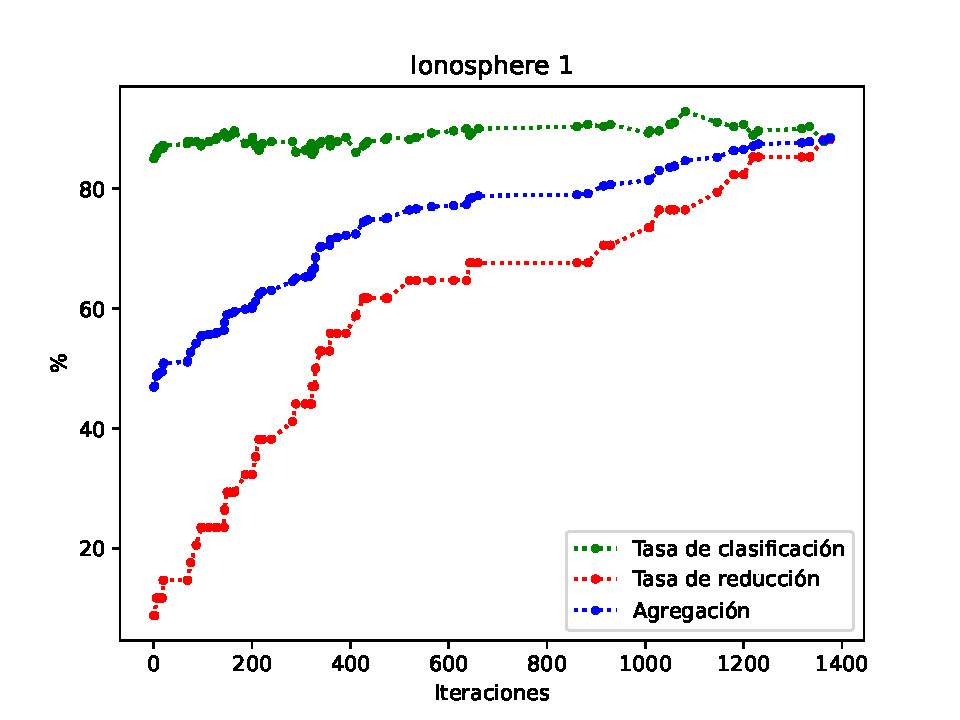
\includegraphics[width=50mm]{../FUENTES/graph/plots/ionosphere1.pdf}}
	\subfigure{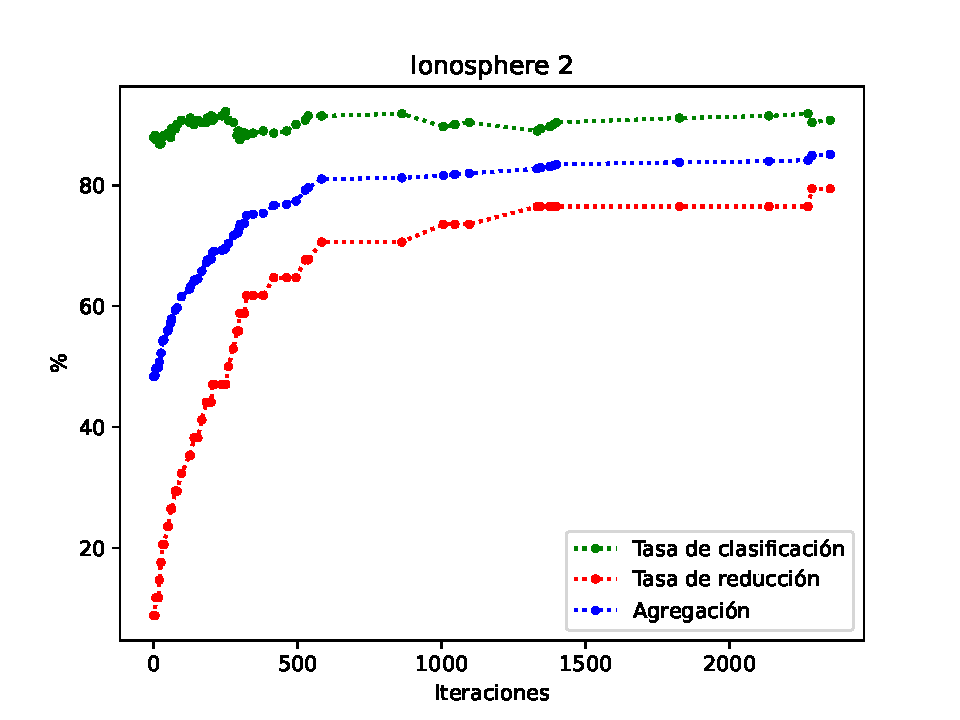
\includegraphics[width=50mm]{../FUENTES/graph/plots/ionosphere2.pdf}}
	\subfigure{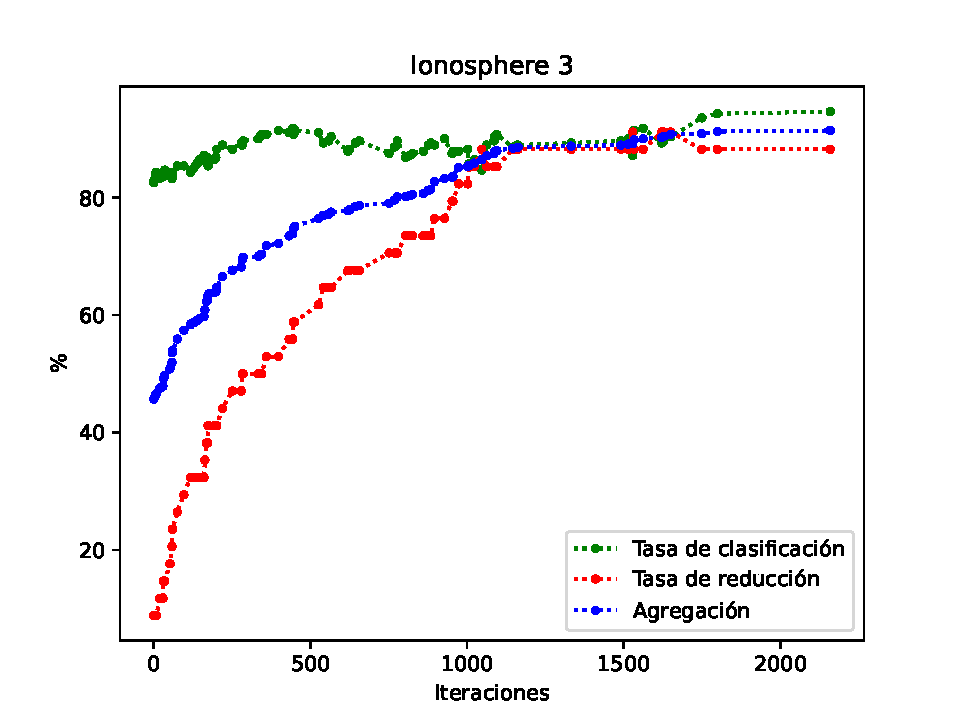
\includegraphics[width=50mm]{../FUENTES/graph/plots/ionosphere3.pdf}}
	\subfigure{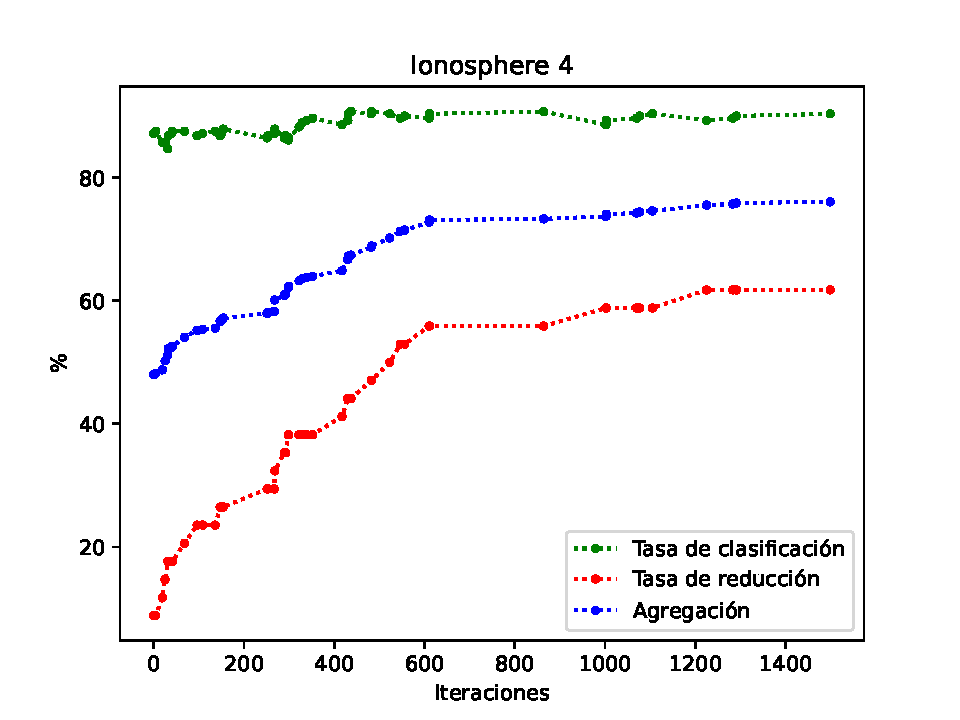
\includegraphics[width=50mm]{../FUENTES/graph/plots/ionosphere4.pdf}}
	\subfigure{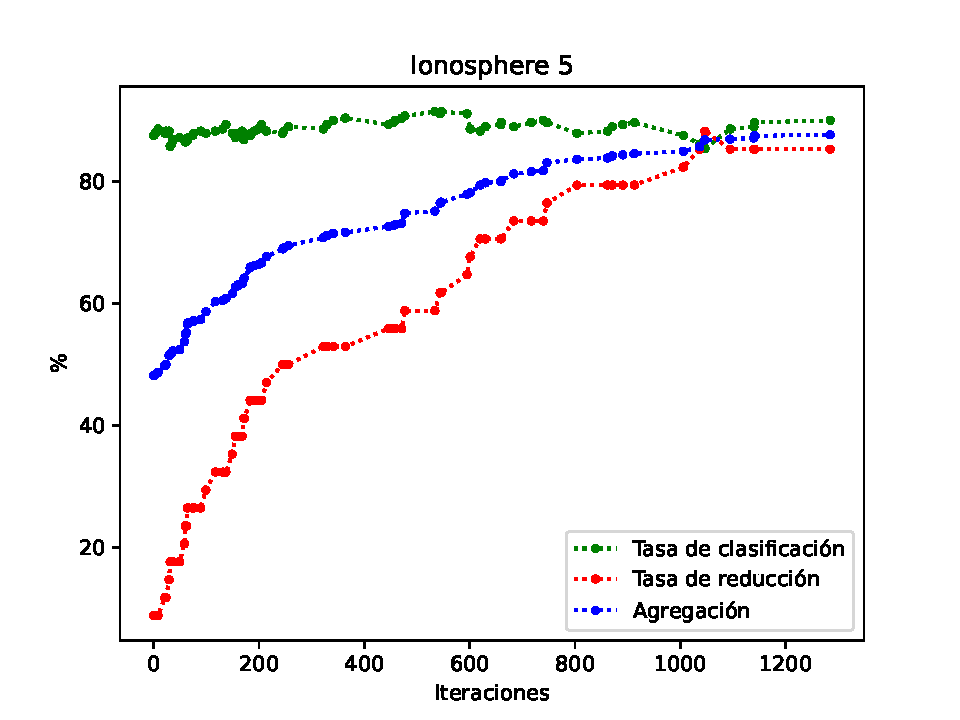
\includegraphics[width=50mm]{../FUENTES/graph/plots/ionosphere5.pdf}}
	\caption{Gráficas de la tasa de clasificación, reducción y agregación respecto al número de iteraciones con los datos de train de Ionosphere}
\end{figure}

\begin{figure}[H]
	\centering
	\subfigure{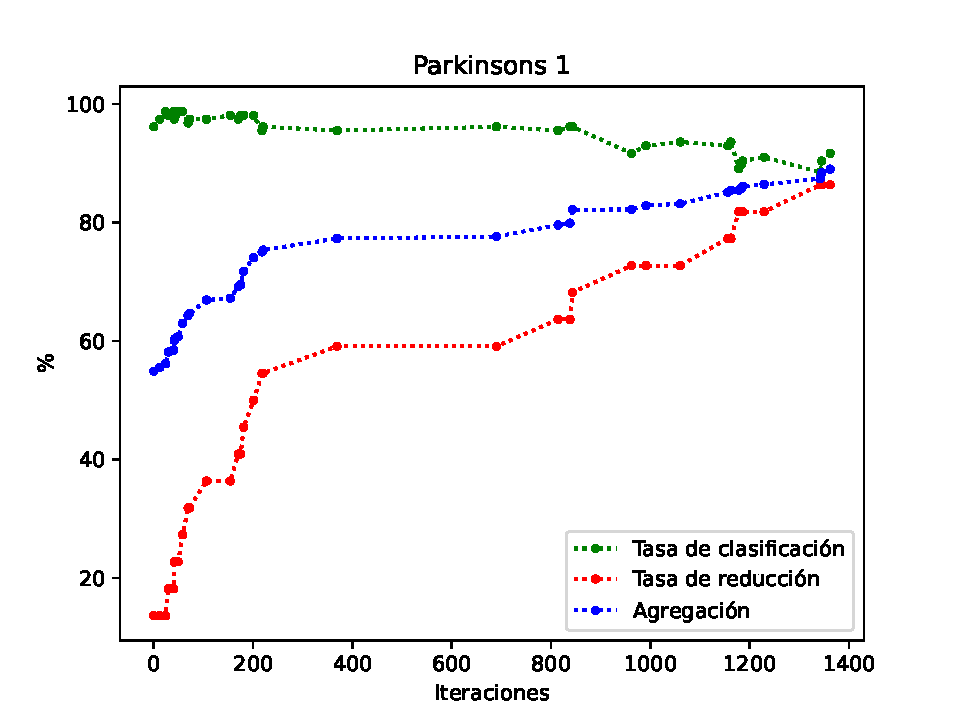
\includegraphics[width=50mm]{../FUENTES/graph/plots/parkinsons1.pdf}}
	\subfigure{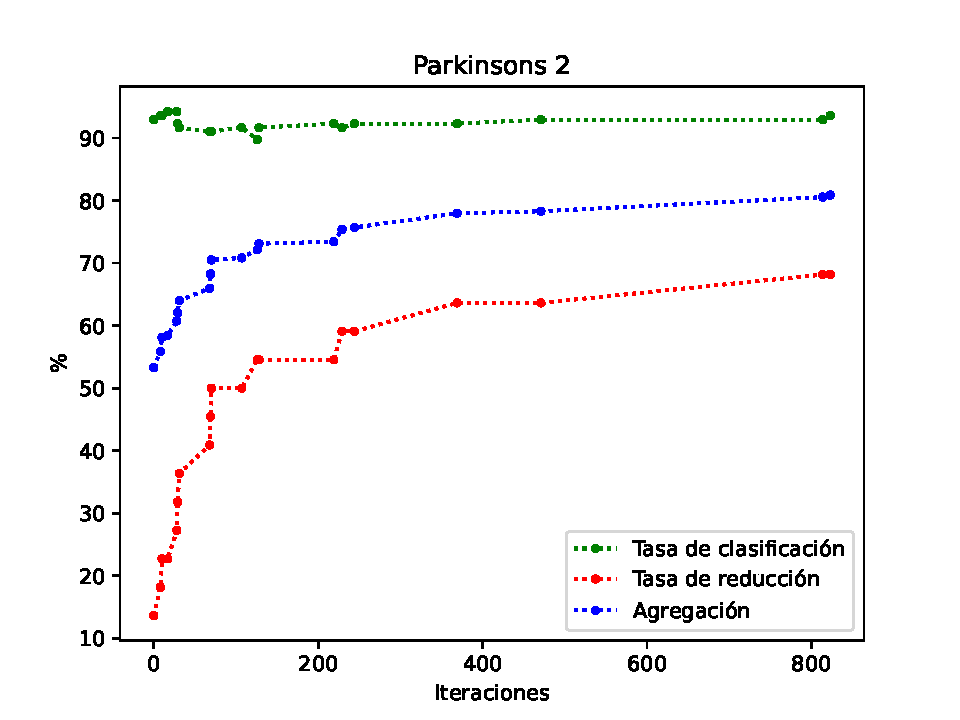
\includegraphics[width=50mm]{../FUENTES/graph/plots/parkinsons2.pdf}}
	\subfigure{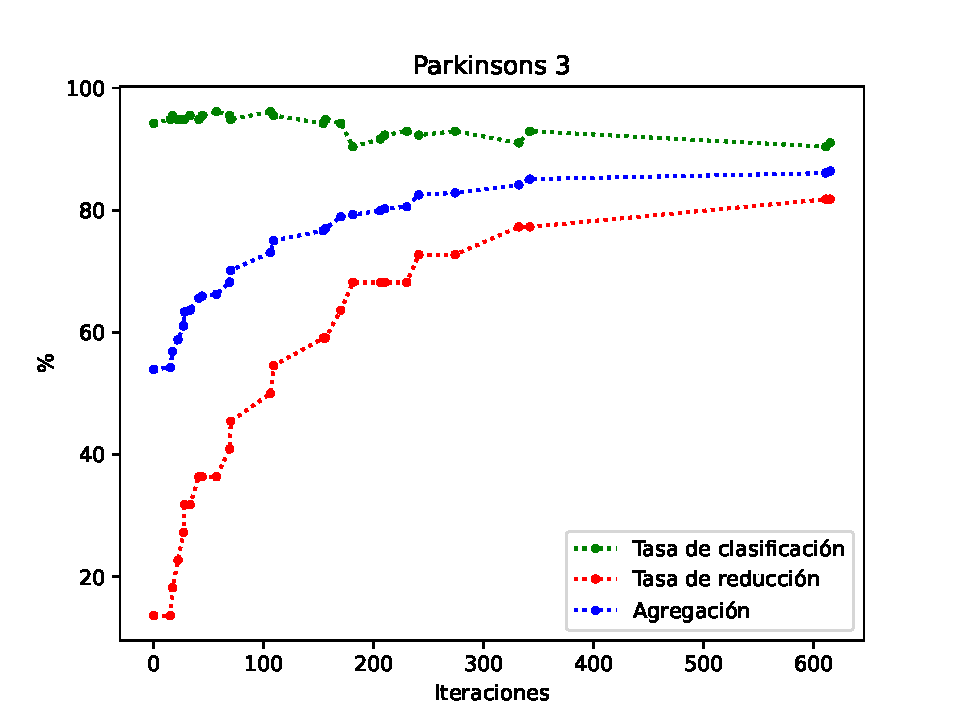
\includegraphics[width=50mm]{../FUENTES/graph/plots/parkinsons3.pdf}}
	\subfigure{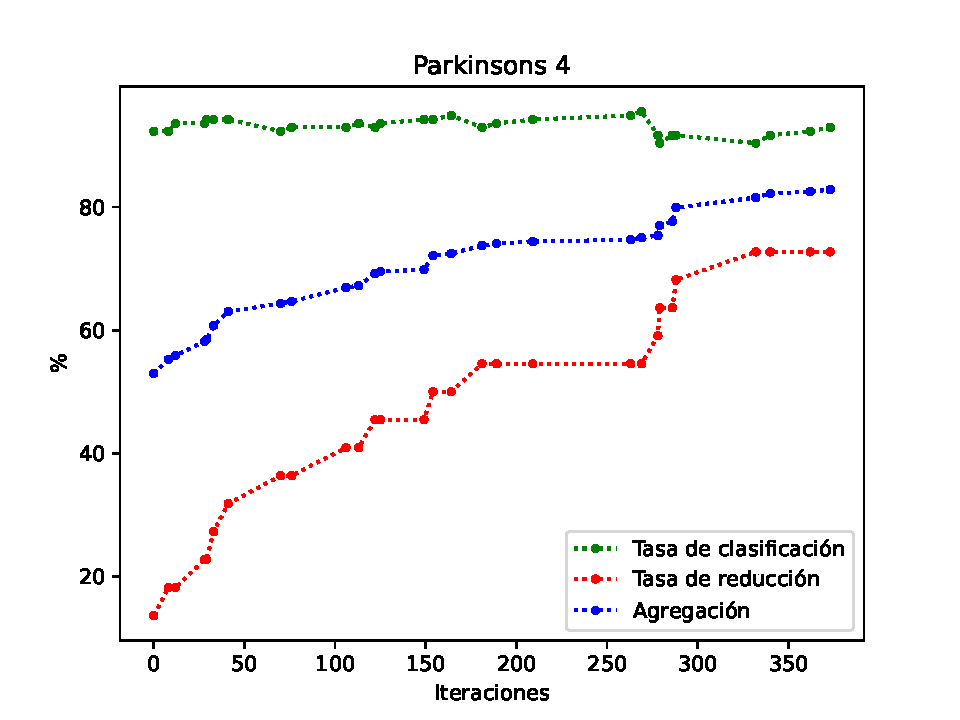
\includegraphics[width=50mm]{../FUENTES/graph/plots/parkinsons4.pdf}}
	\subfigure{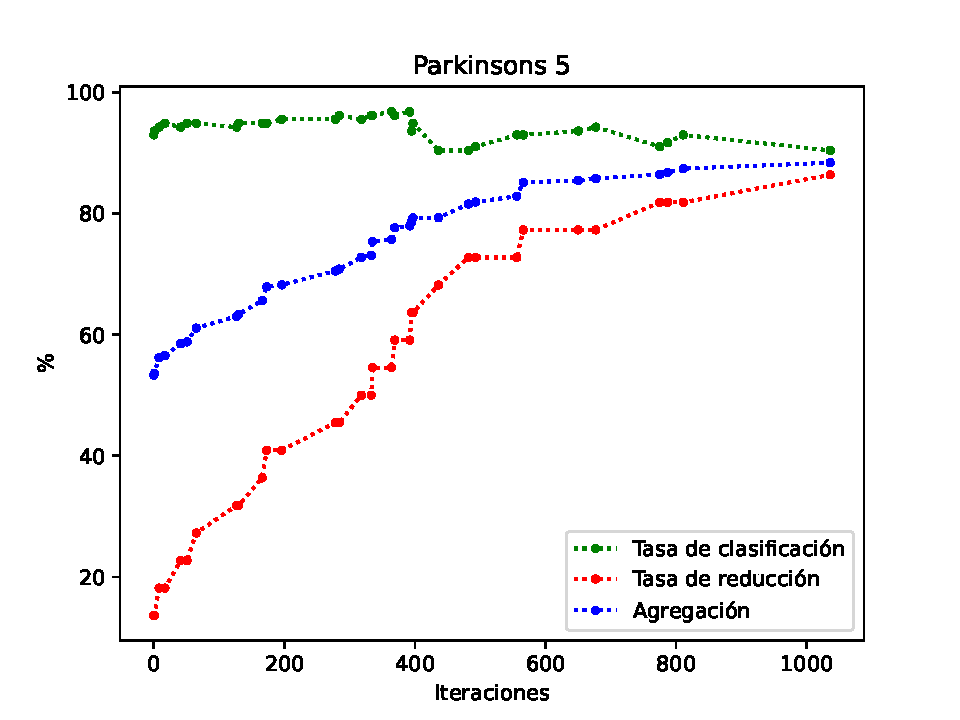
\includegraphics[width=50mm]{../FUENTES/graph/plots/parkinsons5.pdf}}
	\caption{Gráficas de la tasa de clasificación, reducción y agregación respecto al número de iteraciones con los datos de train de Parkinsons}
\end{figure}

\begin{figure}[H]
	\centering
	\subfigure{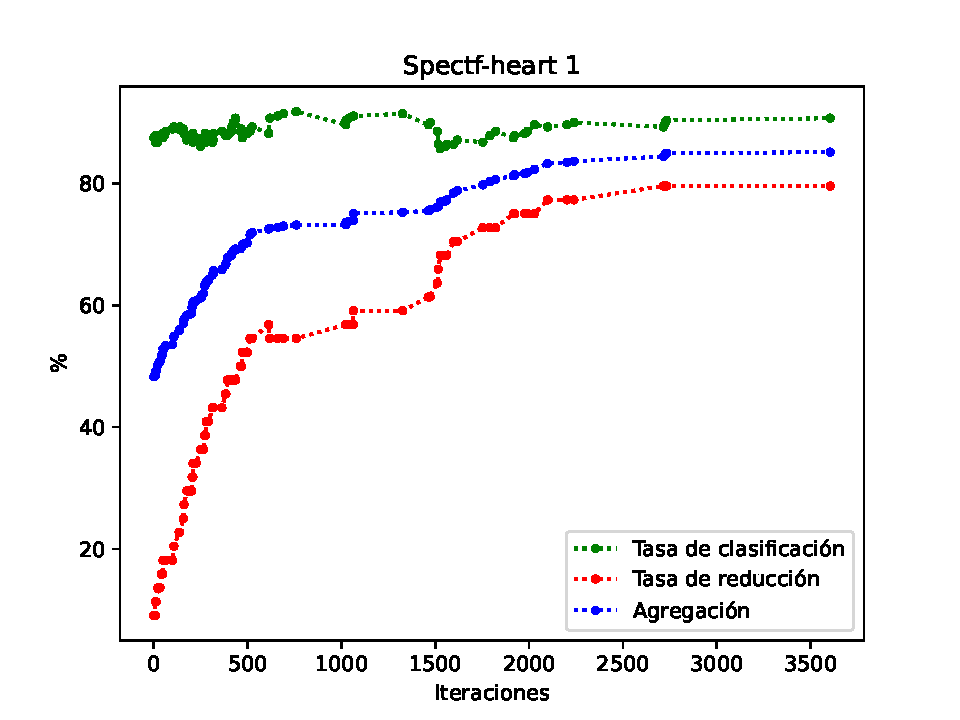
\includegraphics[width=50mm]{../FUENTES/graph/plots/spectf-heart1.pdf}}
	\subfigure{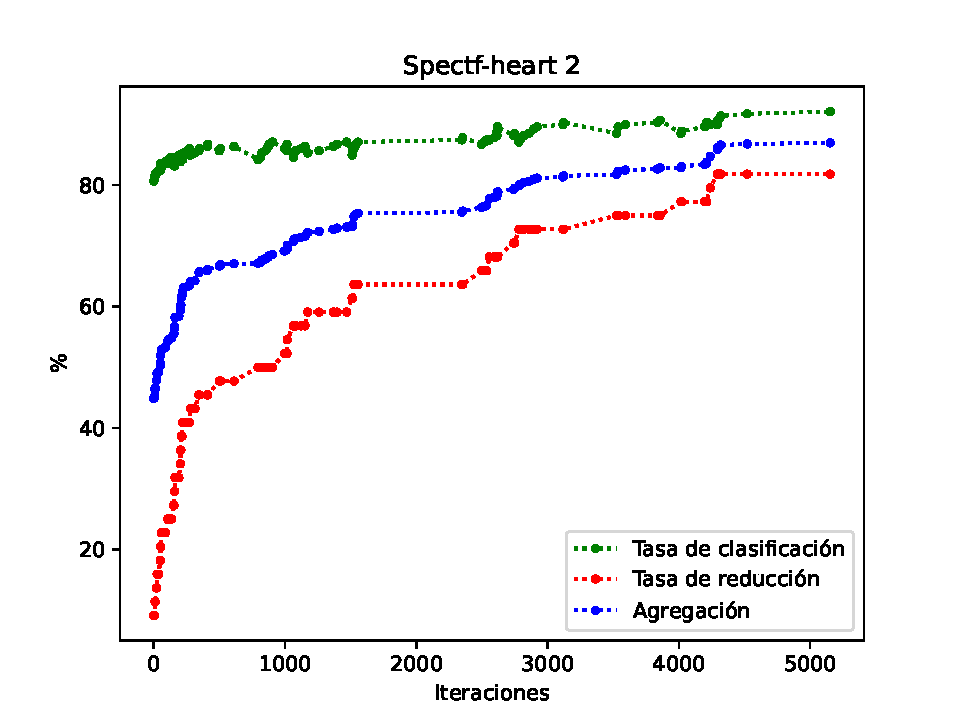
\includegraphics[width=50mm]{../FUENTES/graph/plots/spectf-heart2.pdf}}
	\subfigure{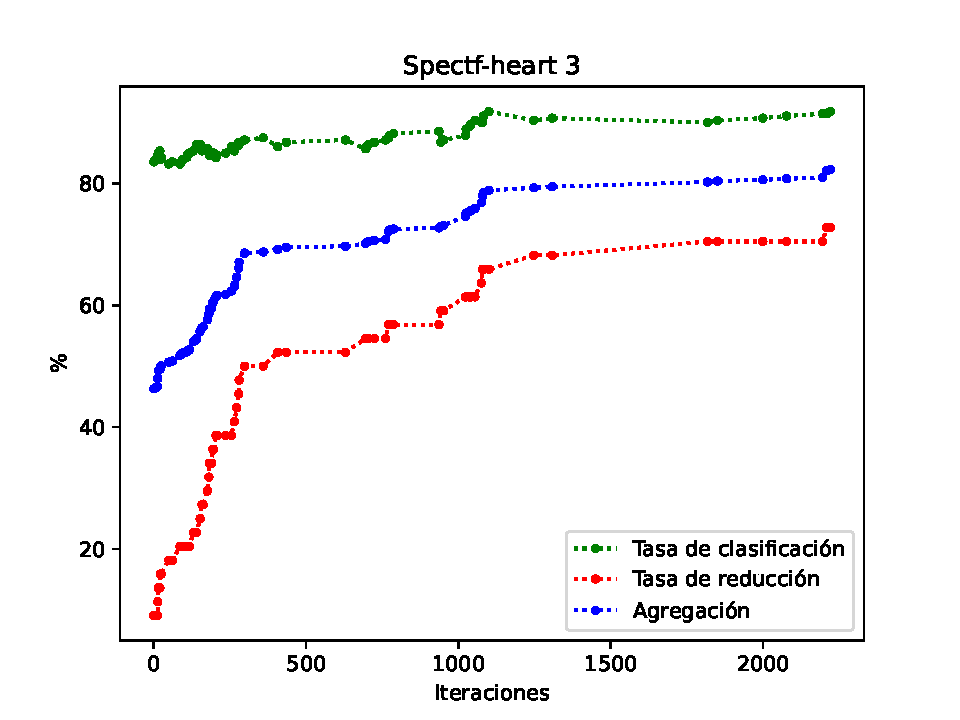
\includegraphics[width=50mm]{../FUENTES/graph/plots/spectf-heart3.pdf}}
	\subfigure{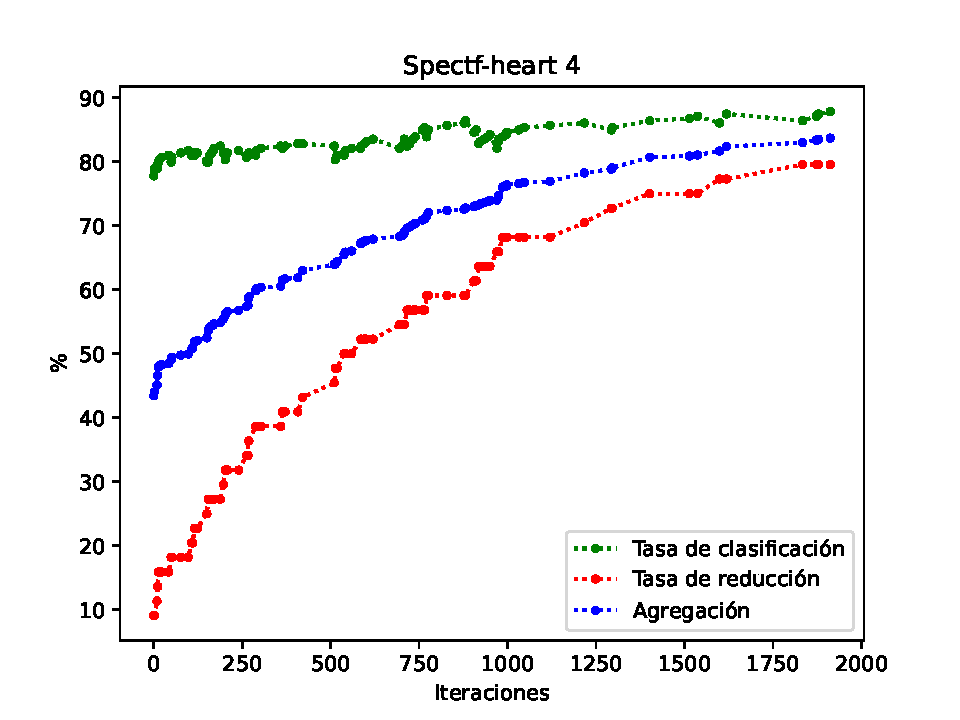
\includegraphics[width=50mm]{../FUENTES/graph/plots/spectf-heart4.pdf}}
	\subfigure{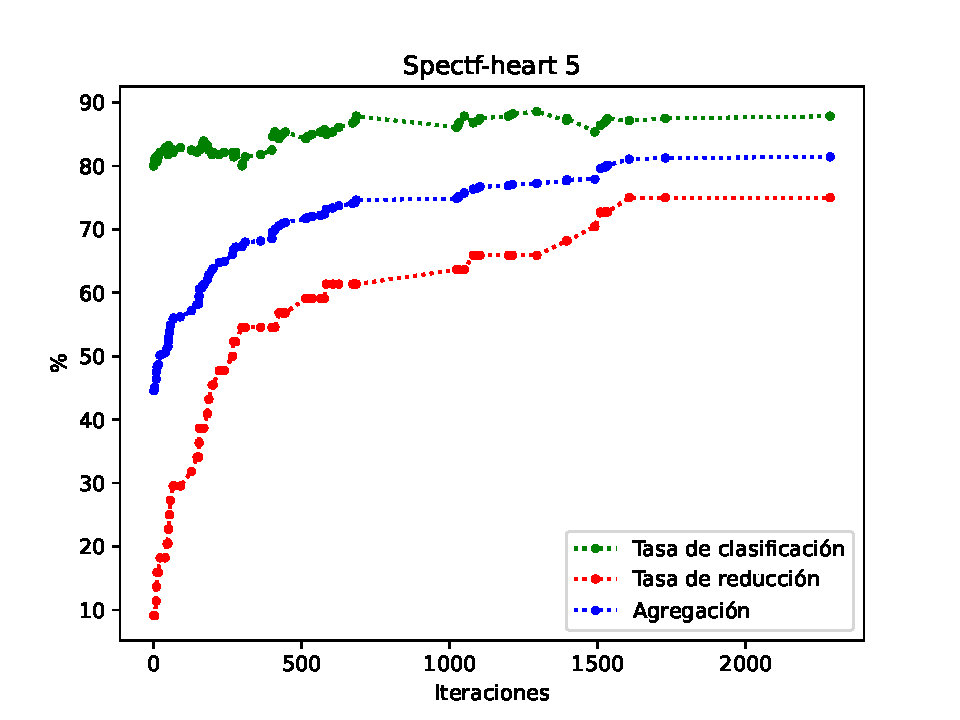
\includegraphics[width=50mm]{../FUENTES/graph/plots/spectf-heart5.pdf}}
	\caption{Gráficas de la tasa de clasificación, reducción y agregación respecto al número de iteraciones con los datos de train de Spectf-heart}
\end{figure}

En todas las gráficas podemos observar los mismos resultados:
\begin{itemize}
\item Inicialmente, la tasa de reducción comienza sobre el 10\%. Esto se debe a que los pesos iniciales siguen una distribución uniforme entre 0 y 1, y eliminamos aquellos que están por debajo de 0.1 por la reducción, los cuáles serán aproximadamente el 10\%.
\item La tasa de evaluación comienza por encima del 50\%, aunque varía en cada caso. Eso se debe a que, aunque esta modificado por unos pesos aleatorios, se sigue usando el algoritmo \emph{1-NN}, por lo que los resultados serán mejor que si los tomásemos completamente al azar (en cuyo caso estarían sobre el 50\% de media).
\item Según aumentan las iteraciones, podemos ver un gran aumento en la tasa de reducción. Esto se debe a que, al empezar cerca del 10\%, tiene un gran margen de mejora, mientras que la tasa de clasificación, al empezar con valores más altos, es más difícil que mejore. Por lo que es mucho más probable una mejora en la tasa de reducción que en la tasa de clasificación.
\item Al aumentar las iteraciones, también vemos como disminuye la pendiente de las gráficas. Esto se debe a que cada vez tenemos mejores soluciones, y es más difícil encontrar una mejora. Inicialmente, hay muchas soluciones mejores, mientras que al final, hay muchas menos al estar cerca del máximo local. Además, no sólo mejora menos en cada paso, si no que es más difícil encontrar una mejor solución, por lo que aumenta el número de iteraciones entre cada punto.
\item Obviamente, al ser tomar $\alpha = 0.5$, la agragación funciona como una media entre la tasa de clasificación y la tasa de reducción, por lo que siempre se encuentra en el punto medio.
\end{itemize}

\subsection{Análisis de los resultados}

Todo este análisis se hace a partir de la tabla \ref{tab:global}.

El algoritmo \emph{1-NN}, como cabe esperar, es con diferencia el más rápido de los tres. Sin embargo, los resultados obtenidos no son muy buenos, principalmente porque no realiza ninguna reducción.

El algoritmo \emph{greedy RELIEF}, aunque siendo mucho más rápido que el algoritmo \emph{localSearch}, es algo más lento que el algoritmo \emph{1-NN}, ya que obtiene tiempos similares con un quinto menos de datos. Sin embargo, los resultados no son mucho mejores, e incluso son peores en algunos casos. Debido a esto, no es un algoritmo que tenga mucho sentido usar en nuestro problema.

El algoritmo \emph{localSearch}, aunque aumenta mucho los tiempos de ejecución, es el algoritmo que da mejores resultados con diferencia. Además, podemos ver como el tiempo crece muy rápido al aumentar las características: teniendo casi el mismo número de ejemplos, pasamos de aproximadamente 32 segundos en \emph{ionosphere.arff} con 34 características a cerca de 52 en \emph{spectf-heart} con 44. Sin embargo, gran parte de estos buenos resultados se debe a la gran reducción que realiza. Debido a esto, hay que tener cuidados de que no produzca un ``sobreajuste'' eliminando demasiadas características.

En resumen, si lo que nos interesa es un algoritmo que tarde poco tiempo, es mejor usar el algoritmo \emph{1-NN}, pero si lo que nos interesa es obtener buenos resultados sin importar el tiempo de ejecución, es mejor el algoritmo \emph{localSeach}.
\end{document}